\documentclass{article}
\usepackage[utf8]{inputenc}
\usepackage[sc]{mathpazo}
\usepackage[dutch]{babel}
\usepackage{hyperref}
\usepackage{enumitem}
\usepackage{pdfpages}
\usepackage[titletoc]{appendix}

\topmargin=-0.45in
\evensidemargin=0in
\oddsidemargin=0in
\textwidth=6.5in
\textheight=9.0in
\headsep=0.25in 


\usepackage{apacite}
\bibliographystyle{apacite}


\title{Portfolio Didactiek}
\author{Fritz van Deventer}
\date{\today}
 
\begin{document}
 
\maketitle

\begin{quote}
  "Maar de boeken spraken met de stem van leraren, of de leraren spraken met de stem van boeken, dat was niet altijd duidelijk. Ze leerden me vaardigheden, maar gaven geen antwoorden."
  \begin{flushright}
    \textit{ - Tommy Wieringa\nocite{speedboot}}
  \end{flushright}
\end{quote}

\tableofcontents

\section{Introductie}
Dit is een portfolio van mij, Fritz van Deventer, geschreven voor de cursus: \textit{HBO didactiek} die wordt gegeven vanuit het HAN VDO instituut van de Hogeschool Arnhem en Nijmegen (HAN).
In dit portfolio komen er in het kort een aantal dingen langs die een beeld geven van wat er geleerd is.

De cursus wordt gegeven aan de hand van 5 onderwerpen: Didactisch creëren, Begeleiden, Ontwerpen, Beoordelen en \textit{Reflective Practicioner}. Voor elk van de eerste vier onderwerpen is er een hoofdstuk bestaand uit een Persoonlijk Ontwikkelingsplan (POP) en een Zelfevaluatie. Het POP eindigt in elk hoofdstuk met een leerdoel geformuleerd uit de observatie van anderen en mijzelf. In iedere Zelfevaluatie blik ik terug op de leerdoelen en beschrijf ik hoe ik aan de leerdoelen heb gewerkt, en in hoeverre ik vind dat deze behaald zijn of niet.

Het laatste onderdeel is verbonden met de andere onderwerpen, maar was niet een afzonderlijk gedeelte in de cursus. Dat is het gedeelte \hyperref[sec:RP]{Reflective Practicioner}. Dit is een onderzoek vanuit de onderwijspraktijk, gebruikmakende van kennis van collega's en gesprekken met studenten. Het onderzoek draait om een vraag die ik het liefst beantwoord zie voor mijn dagelijkse beroepspraktijk namelijk: "Hoe verschillend zijn de zienswijze van student en docent ten opizchte van onderwijs en de rol van de docent daarin?".


\section{Activerende Didactiek}
\subsection{Persoonlijk Ontwikkelingsplan}
\label{sec:didactiek}

Aan de hand van mijn worst-case scenario en een SWOT-analyse heb ik een leerdoel ontwikkeld. De SWOT-analyse is uitgewerkt in \hyperref[tab:SWOTDidactiek]{Tabel 1}.

De SWOT-analyse is opgebouwd uit feedback die ik heb gekregen van anderen, uit dingen die naar voren zijn gekomen in de lesbezoeken, de lesdemo en een aha-erlebnis die ik uit mijn worst-case scenario heb gehaald.


\begin{table}[h]
  \begin{center}
  \hspace*{-2cm}
  \begin{tabular}{ l | p{6cm} | p{6cm} }
     \hline
      & behulpzaam & schadelijk \\ \hline
     intern & 
       \begin{itemize}[noitemsep, leftmargin=*]
         \item{Gebruik van voorbeelden en metaforen} 
         \item{Zekere indruk.}
         \item{Vragen positief bekrachtigen met complimenten.}
         \item{Laagdrempelig}
         \item{Heldere duidelijke stem. Prettig aanwezig}
       \end{itemize}
     & 
       \begin{itemize}[noitemsep, leftmargin=*]
         \item{Te weinig tijd geven voor een antwoord}
         \item{De belangrijke dingen verbaliseer ik te weinig.}
         \item{Niet rekening houden met andere leerstijlen.}
         \item{Te weinig context bieden, bij een sprong in het diepe.}
         \item{Niet genoeg tijd nemen voor lesvoorbereiding.}
       \end{itemize}
         \\ \hline
     extern & 
       \begin{itemize}[noitemsep, leftmargin=*]
         \item{Over het algemeen is er genoeg tijd om lessen voor te bereiden, waarmee er ook een diversiteit in werkvormen valt te onderzoeken.
         \item De lessen zijn allemaal lang (3 uur), hierin is genoeg tijd om context te geven rond een thema, een werkvorm te doen en daarop te reflecteren tijdens de les.}
       \end{itemize}
       & 
       \begin{itemize}[noitemsep, leftmargin=*]
         \item{Iedereen zit in de les met een laptop voor hun neus, de kans tot afleiding is en de kans dat dingen mij ontgaan die de klas bezighouden zijn groot.}
         \item{De afstand tussen de student en mij in jaren groeit.}
       \end{itemize}
       \\
     \hline
   \end{tabular}
   \caption{SWOT analyse. Met de klok mee: S, W, T, O.}
   \label{tab:SWOTDidactiek}
  \end{center}
 \end{table}

\subsubsection{Worst-case scenario}
De worst-case is voorgevallen op een middelbare school waar ik lesgaf aan een VWO 5 klas. Richting het einde van het jaar was er een hoofdstuk wat inzoomde op de geschiedenis van Informatica. Daarmee werd het minder een oefening van nieuwe vaardigheden zoals dat met andere onderwerpen zoals programmeren en databases wel het geval was. Maar vooral een kwestie van begrijpend lezen en het onthouden van wat feiten.

De stof zelf was niet heel inspirerend, dat was misschien ook wel duidelijk af te lezen aan mijn houding. Daarenboven had ik mijn lessen niet altijd goed voorbereid met een onderbreking of iets leuks. Om de powerpoints en de stof op te leuken, had ik hier en daar een filmpje ter ondersteuning gezocht. Wat grapjes en wat anecdotes om de slides te ondersteunen. Helaas was de desbetreffende les een tranendal. Gedurende een 20 minuten durende presentatie, werd het steeds rumoeriger en begon ik steeds meer tegen de ruggen dan tegen de gezichten van de leerlingen aan te kijken. Ik maakte even een zijstapje. Ik parafraseer:
\begin{quote}
  \textit{"Wat gebeurt er precies? Ik snap dat dit misschien niet het meest interessante onderwerp is en dat het bijna vakantie is. We doen dit samen, als jullie meedoen gaat het een stuk sneller."}
\end{quote}

Vervolgens werd er 1 minuut stilte geveinsd waarna de houding van daarvoor weer een schepje er bovenop kreeg. Op dat moment werd ik zelf wat sarcastisch en begon snel door de slides heen te klikken waarbij ik dingen riep als: \textit{"Kijk, een plaatje. leuk hé?"}. Dit schouwspel verstomde de klas tot een allesomvattende stilte, waarbij ik het eindigde met: \textit{"Ik haal even koffie."}

Daarna heb ik mijzelf vermand, het was een blokuur en de bel van het eerste van de twee uur was nog niet gegaan. Toen heb ik wat interessante dingetjes opgezocht een kahoot gemaakt en wat rondgelopen om leerlingen te praten over hun buitenlandexcursie.

Wat mij hierin opviel is dat ik het heel vervelend vond dat ik totaal de aandacht en het contact met leerlingen was verloren. Wat eigenlijk het hele jaar goed was gegaan als beginnende docent liep nu finaal in de soep. Dit verwijt ik grotendeels mijzelf. Door het onderwijs inmiddels iets bewuster te begrijpen vanuit onderwijsfuncties \cite[p.45-62]{kallenberg2014leren} zie ik dat ik qua cognitie en affect redelijk vanuit instinct heb kunnen handelen. Maar het ontbreekt mij nog aan regulatieve maatregelen die iets meer proces en structuur aan de lessen geven. Om die verschillende onderwijsfuncties bewuster in te vullen wil ik gebruik maken van het lesplan, dat de verschillende fasen van een les onderverdeeld en taken definieert die passen binnen de verschillende onderwijsfuncties en tracht te voorkomen dat belangrijke didactische stappen worden overgeslagen \cite[p.163-169]{bijkerk2015activerend}.
%Deze stof had ik zelf niet iets leuks van gemaakt. Waar dat misschien wel mogelijk was. Hierin zat mijn grootste falen in de voorbereiding. Ik bereid niet altijd mijn lessen goed voor, waardoor ik soms aangewezen ben op mijn improvisatievaardigheden. Door deze worst-case te ondergaan ben ik er van overtuigd dat ik zelfs de lessen die mij makkelijk af zouden moeten gaan gedegen moet voorbereiden.

\subsubsection{Leerdoel}
Het leerdoel wat ik uit de SWOT-analyse en de worst-case scenario heb gedistilleerd is als volgt:
\begin{quote}
  De lessen en lesstof die mij minder interesseren ga ik meer aandacht geven dan de lesstof die \textit{"leuk"} is.
\end{quote}

Dit leerdoel wil ik gaan behalen door voor de eerste 4 lessen van het nieuwe blok (P1 2017/2018) een planning te maken aan de hand van het lesplan. Hiermee dwing ik mijzelf om wat ruimer van te voren de tijd te nemen om over mijn les na te denken. In de hoofdfase van de les wil ik dan graag gebruik maken van verschillende activerende werkvormen die om het leren op gang te brengen het leren combineren met het opdoen van concrete ervaringen zoals in de leercyclus van Kolb \cite[p.143-145]{kallenberg2014leren}. 

\subsection{Zelfreflectie}
\label{sec:Zelfreflectie}
Hier zal ik terugblikken op het leerdoel welke ik heb geformuleerd en hoe ik dat heb getracht te behalen. De reflecties zowel als de feedback formulieren van de lesdemo en het lesbezoek van de docent staan in Bijlage \hyperref[sec:lesdemo]{A}, \hyperref[sec:lesbezoek]{B} en \hyperref[sec:lesbezoekcollega]{C}..

De afgelopen 4 lessen heb ik nu met behulp van het lesplan vormgegeven, wat een hele uitdaging bleek, want structureren gaat bij mij niet zo vanzelf. Ik ben vrij goed in improviseren en vertrouw er dan ook op dat ik als een onderdeel minder goed heb voorbereid, dat ik er dan ook wel uitkom zonder die voorbereiding. Dat is een sterke kant van mij, maar niet een kant die ik wil misbruiken in dienst van mijn eigen luiheid. Het voordeel is dat wanneer zich een onvoorziene situatie voordoet dat ik die goed kan anticiperen en daarop handelen. Het nadeel is echter dat ik niet altijd duidelijk heb wat ik de studenten precies wil meegeven en hoe ik dat ga doen.
Als ik dat niet goed voorbereid dan ben ik zo bezig met improviseren dat ik dan te weinig ondertitel van wat we doen en waarom we dat doen in de les. Wat precies dat regulatieve gedeelte in het gevaar brengt.

Toen ik bezig ging met het lesplan tijdens de cursus zag ik daar wel wat het voordeel er van zou kunnen zijn. Maar in de dagelijkse praktijk voelt dat omslachtig. Eerst een lesplan en van daaruit een les voorbereiden.

Desalniettemin ben ik er mee aan de slag gegaan voor mijn leerdoel. Ik ben elke voorbereiding gestart met het rudimentair opschrijven van het doel, de orde van leren die het doel tracht te behalen volgens de taxonomie van Bloom en de methoden aan de hand van de lesinhoud. Tijdens de voorbereiding begon ik dan ook wat slides te maken om de les wat te omlijsten. Dat alleen al gaf een kapstop om de les in te delen. De hulpwoorden: \textit{duo's, plenair, carousel} hielpen mij om in ieder geval iets anders te bedenken dan een individueel of plenair deel. Hiermee heb ik kunnen oefenen met wat verschillende activerende werkvormen. Zo heb ik de studenten aan elkaar laten verwoorden welke nieuwe concepten ze de voorgaande lessen hebben geleerd en hoe ze die kunnen gebruiken. Of kleine opdrachten gegeven die analoog zijn aan de resultaten die worden verwacht bij het uiteindelijke beroepsproduct van het vak. Zo hebben ze tijdens de les een programma moeten maken dat een dambord met damstukken tekent. Dit sluit ook aan bij de handelingspsychologie leertheorie \cite[p.417]{kallenberg2014leren}. Die stelt dat het leren bestaat uit een materiële (denk aan het dambord), een perceptieve (zoek het dambord op op internet), verbale (beschrijf aan elkaar waar een dambord uit bestaat) en een mentale handeling (aan welke regels voldoet een dambord). 

In vrijwel elke les verwerk ik een kleine competitieve quiz met Kahoot, waarbij ik de stof van vorige week ophaal door middel van vragen te stellen met code-voorbeelden. Eenmaal in de week zijn de studenten zelf aan de beurt om vragen te maken. Ten eerste vinden ze het heel leuk dat hun eigen vraag langskomt, dus zijn ze volledig geëngageerd en ze oefenen nogmaals met het formuleren van hun kennis, wat ook als 1 van de top-strategieeen van het leren wordt genoemd in: \textit{"What Works, What Doesn't?"} \cite{dunlosky2013}.

Het gebruiken van activerende werkvormen wordt steeds gemakkelijker om vanzelf op te pakken. De \textit{grabbelton van ervaring} wordt steeds rijkelijker gevuld en is in dat opzicht weer complementair aan mijn improvisatievaardigheden.

Door het lesplan te gebruiken, denk ik van te voren na over wat ik welk leerresultaat ik beoog. Ik denk er over na waar ik mee wil beginnen en wat ik wil behandelen. Al met al ben ik heel blij met mijn gekozen leerdoel en hoe het is uitgepakt. Om heel eerlijk te zijn verwacht ik niet elke les met behulp van het lesplan te gaan voorbereiden, maar het helpt mij in ieder geval aan het begin van een nieuw vak om wat richting te geven in hoe ik mijn les indeel en wat ik erbij pak.
Waar ik nog steeds te kort in schiet desondanks het gebruik van het leerplan is de afsluiting. Ik heb gemerkt dat ik niet altijd goed terugkoppel wat we hebben behandeld, ik blik niet terug op de leerdoelen en kom daar verder weinig op terug. Dat zou ik graag in de toekomst willen veranderen door de komende 3 lessen juist op dat laatste stuk van de les te focussen in de voorbereiding. Maar de evaluatie daarvan is helaas niet bestemd voor dit document.

\subsection{Ontvangst}
Aan het eind van elk vak wordt er een docentenevaluatie afgenomen. In deze evaluatie komt naar voren dat de studenten zeer tevreden zijn geweest met mijn lessen, ik denk dat ook ten dele komt door de extra voorbereiding die ik erin heb gestopt. Hieronder zijn de resultaten te vinden van die evaluatie.
\begin{table}[h]
  \begin{center}
  \hspace*{-2cm}
  \begin{tabular}{ l | p{10cm} | p{2cm} }
    
    1. & Deze docent is vakinhoudelijk deskundig & 4.86	 \\
    2. & Deze docent is didactisch vaardig	& 4.9 \\
    3. & Deze docent heeft voldoende kennis van de beroepspraktijk	 & 4.43 \\
    4. & De bijeenkomsten van deze docent ervaar ik als zinvol & 4.85 \\ 
    5. & Deze docent toont zich in studenten geïnteresseerd & 4.8 \\
    6. & Ik kan zonder problemen met mijn vragen bij deze docent terecht & 4.8 \\
    7. & Deze docent geeft bruikbare feedback op mijn leerprestaties & 4.5 \\
    8. & Deze docent inspireert / motiveert mij om een goede beroepsbeoefenaar te worden	& 4.45 \\
  \end{tabular}
  \caption{Docentenevaluatie vak SPD.}
  \label{tab:docentenevaluatie}
  \end{center}
\end{table}

\begin{itemize}
  \item Docent is zeer gericht op de lesstof die voor de huidige week staat gepland. Uitlopers krijgen minder feedback op hun opdrachten.
  \item Erg jong, erg slim, leuk om naar te luisteren, legt duidelijk de stof uit en had de eerste dag van les geven al alle namen van onze klas in zijn hoofd, heel erg betrokken en aardig!
  \item Geen opmerkingen, Fritz is een gemotiveerde docent en je kunt bij Fritz veel leren.
  \item Goede leraar, legt goed en duidelijk uit.
  \item Frits is mijn idee van een perfecte docent
  \item Goede docent! Legt duidelijk uit en blijft herhalen en vragen of het duidelijk is
\end{itemize}

% Om tot een goed leerdoel te komen, heb ik gebruik gemaakt van een SWOT matrix (zie Tabel~\ref{tab:SWOTDidactiek}), waarin ik Strengths (S), Weaknesses (W), Opportunities(O) en Threats(T) heb ingedeeld op behulpzaam (SO) en schadelijk (WT) en intern (SW) en extern (OT). Met intern bedoel ik de dingen in mij zelf, waar ik zelf invloed op kan uitoefenen en met extern de dingen die vanuit anderen komen en waar ik minder invloed op kan uitoefenen. 




\section{Begeleiden}
\subsection{Persoonlijk Ontwikkelingsplan}

Bij het begeleiden van stages en afstuderen merk ik dat ik veel op zoek ben naar \textit{een verdieping} van het werk, die nog ontbreekt. Bijvoorbeeld: De student start een onderzoek van 6 maanden maar heeft een onderzoeksvraag die in een week opgelost kan zijn. Niet iedereen doet dit automatisch goed. Dat is ook niet vreemd, niet alle studenten ontwikkelen zich hetzelfde. Ik wil graag daarin gebruik maken van de psychologische ontwikkelingsstadia, omdat die een redelijk goede indicator blijken voor het inschatten van plannings- en andere zelfregulatievaardigheden \cite{luken2008mogelijkheid}. Maar ik merk dat ik schipper tussen de verantwoordelijkheid bij de student laten en soms te veel invullen of doen voor de student. Dan wil ik de gesprekstechnieken, zoals het GROW-model toepassen om te kijken of er een betere onderzoeksvraag boven tafel kan komen.

Mijn leerdoel wordt dus:
In het komende contact voor een afstudeer- en/of stagebegeleiding wil ik door middel van gebruik van het GROW-model komen tot een verdieping voor de student, vooral als de student zelf niet in staat lijkt tot zelfregulatie. Een verdieping kan dan zijn: een realistischere planning, een betere onderzoeksvraag of iets dergelijks.

Hieronder beschrijf ik twee situaties, één van een individuele begeleiding en één van een groepsbegeleiding. Hierna beschrijf ik hoe het contact vond gaan en probeer ik in te zoomen op hoe ik mijn leerdoel heb getracht te proberen te halen.

\subsection{Situatieschets Individuele begeleiding}
\label{sec:individu}
Één van de studenten die ik begeleid voor zijn afstuderen had een projectplan opgestuurd wat nogal onder de maat was. Erg algemene risico's niet echt specifieke doelen om te behalen en onderzoeksvraag waar niet echt mee gewerkt kon worden. Naar aanleiding van zijn projectplan en om even kennis te maken met de student, het afstudeerbedrijf en zijn begeleiders had ik een afspraak gemaakt met hem.

De afspraak begon helaas een beetje scheef omdat ik vergeten was de feedback die ik voor hem had verzameld een aantal dagen voor de afspraak naar hem te sturen. De student was een beetje verrast door mijn terugkoppeling op zijn document en de onderdelen die ik nog te onduidelijk vond. Het overviel hem even op dat moment, dat was totaal niet mijn bedoeling. 

Daarna heb ik geprobeerd door wat vragen te stellen duidelijker te krijgen wat de situatie was en wat de doelstelling van de opdracht was. Op een gegeven moment heb ik het gesprek afgerond en voorgesteld om nog even met de student individueel te zitten en samen te kijken naar de onderzoeksvraag en het werk wat er nog moet gebeuren.

De gesprekstechnieken die besproken zijn in de lessen en de oefening met de acteur waren mij allemaal even ontschoten en het kostte mij redelijk wat tijd om die weer op orde te krijgen. De taak als begeleider is naar mijn idee om de student zelf aan het denken te zetten. Op het moment dat de situatie dan geheel anders loopt, doordat de student de feedback pas voor het eerst hoorde toen ik bij hem was, dan is het toch een stuk lastiger om het ook daadwerkelijk bij de student te laten en niet zelf heel hard te gaan werken. 

Gezamenlijk hadden we afgesproken om elkaar nog telefonisch te spreken over het projectplan een week later. Tijdens dat gesprek was het een stuk makkelijker om de "goede" vragen te stellen en de student aan het werk te zetten. Hier blijkt voor mij duidelijk uit dat het belangrijk is om die gesprekstechnieken veelvuldiger te oefenen en te gebruiken zodat het een tweede natuur wordt, ook voor de onvoorziene situaties.


\subsection{Situatieschets Groepsbegeleiding}
\label{sec:groep}
\subsubsection{Context}
In het eerstejaars project van de Informatica opleiding (I-Project) ben ik procesbegeleider geweest van een groep studenten die een veilingssite moesten maken voor een opdrachtgever (een rol die vervuld werd door een andere docent). De casus en de inhoud van de opdracht waren weggelegd voor de opdrachtgever. Het was belangrijk dat het groepje waar ik begeleiding aan gaf bekend zou worden met de procestool: \textit{Scrum}. Scrum is een manier van werken in teamverband waar er getracht wordt kleine iteraties te maken die elk afgerond worden met een product wat af is. In de praktijk betekent dit veelal het afspreken, plannen en opleveren van de beloofde dingen voor een product in een tijdsperiode van een aantal weken, een zogenoemde \textit{sprint}. Na afloop van elke sprint is er normaliter een \textit{retrospective}, een overleg met elkaar om terug te blikken op hoe het samenwerken gegaan is. Naast dit overleg kwam ik regelmatig langs om even te kijken hoe het ging (en of iedereen wel aanwezig is).

\subsubsection{Situatie}
In de groepsgesprekken gaf ik meestal een taak mee voor het volgende ontmoetingsmoment. De opdracht die ik gegeven had voor dit specifieke gesprek was om feedback op te schrijven voor elk van de groepsleden, een tip en een top. De opdracht had ik gegeven omdat in sommige van de gesprekken daarvoor ze ook de taak hadden om feedback mee te nemen, maar de meesten deden het uit het hoofd en het leek nogal verzonnen ``on-the-spot'', het had weinig diepgang en iedereen ging elkaar wat napraten. Ik had nadrukkelijk genoemd dat iedereen echt wat moest opschrijven, anders zou ik zelf weglopen bij het gesprek, omdat het dan ook geen zin had om feedback met elkaar te bespreken.

De volgende afspraak had iedereen wat opgeschreven en meegenomen. Toen we de ronde deden was een van de leden van de groep (we geven hem even de fictieve naam: Hendrikus) nog steeds terughoudend met het geven van de tip. Hendrikus noemde steeds dat de anderen het zo goed doen en dat hij er niet echt iets had op aan te merken. Op dat moment leek het mij verstandig om een zijstapje te doen en te communiceren over het communiceren met de groep. Ik vroeg ze of ze het prima vonden als Hendrikus iets over hun zou zeggen waar ze aan moesten werken of wat niet louter positief was. De groep antwoordde dat ze daar echt niet bang voor waren, dit verwoordde ze ook naar Hendrikus, dat hij zich daar niet zorgen over hoefde te maken. Ik vroeg ook Hendrikus of hij misschien wist waarom hij het niet zo goed over zijn lippen kreeg. Had hij dan geen feedback? Of vond hij het spannend? 

Op dat moment leek het alsof er even een schilletje om Hendrikus wegviel. Hij noemde dat hij het inderdaad ingewikkeld vond om iets negatiefs (ook al was het opbouwend bedoeld) te zeggen omdat hij in zijn schoolloopbaan redelijk veel gepest werd. Hij was bang dat hij het vertrouwen of zijn goede band met de anderen zou schaden door iets te noemen wat niet positief was. Nadat hij dit noemde reageerde de groep accepterend en herhaalde nogmaals dat hij zich er niet zorgen om hoefde te maken. Waarna Hendrikus ook zijn tips durfde te delen.

Wat ik merkte in dit gesprek is dat het echt wel loont om soms even een zijstap te doen en te durven door te vragen. Wat er nog wel bij gezegd moet worden, is dat in deze groep een andere jongen de groep heeft moeten verlaten die kampte met depressie in combinatie met een Autisme Spectrum stoornis.

% \subsection{Situatieschets Individuele begeleiding}
% \label{sec:individu}
% Één van de studenten die ik begeleid voor zijn afstuderen had een projectplan opgestuurd wat nogal onder de maat was. Erg algemene risico's niet echt specifieke doelen om te behalen en onderzoeksvraag waar niet echt mee gewerkt kon worden. Naar aanleiding van zijn projectplan en om even kennis te maken met de student, het afstudeerbedrijf en zijn begeleiders had ik een afspraak gemaakt met hem.

% De afspraak begon helaas een beetje scheef omdat ik vergeten was de feedback die ik voor hem had verzameld een aantal dagen voor de afspraak naar hem te sturen. De student was een beetje verrast door mijn terugkoppeling op zijn document en de onderdelen die ik nog te onduidelijk vond. Het overviel hem even op dat moment, dat was totaal niet mijn bedoeling. 

% Daarna heb ik geprobeerd door wat vragen te stellen duidelijker te krijgen wat de situatie was en wat de doelstelling van de opdracht was. Op een gegeven moment heb ik het gesprek afgerond en voorgesteld om nog even met de student individueel te zitten en samen te kijken naar de onderzoeksvraag en het werk wat er nog moet gebeuren.

% De gesprekstechnieken die besproken zijn in de lessen en de oefening met de acteur waren mij allemaal even ontschoten en het kostte mij redelijk wat tijd om die weer op orde te krijgen. De taak als begeleider is naar mijn idee om de student zelf aan het denken te zetten. Op het moment dat de situatie dan geheel anders loopt, doordat de student de feedback pas voor het eerst hoorde toen ik bij hem was, dan is het toch een stuk lastiger om het ook daadwerkelijk bij de student te laten en niet zelf heel hard te gaan werken. 

% Gezamenlijk hadden we afgesproken om elkaar nog telefonisch te spreken over het projectplan een week later. Tijdens dat gesprek was het een stuk makkelijker om de "goede" vragen te stellen en de student aan het werk te zetten. Hier blijkt voor mij duidelijk uit dat het belangrijk is om die gesprekstechnieken veelvuldiger te oefenen en te gebruiken zodat het een tweede natuur wordt, ook voor de onvoorziene situaties.

\subsection{Zelfreflectie}
In de gedeelten \hyperref[sec:groep]{Situatieschets Individuele begeleiding} en \hyperref[sec:individu]{Situatieschets Groepsbegeleiding} worden twee situaties aangedragen. Allereerst zou ik even de individuele situatie van de afstudeerder even willen uitlichten aan de hand van het estafetteloop-model \cite{methorstkaders}. Daarna behandel ik de groepssituatie aan de verschillende niveaus van reflectie van Korthagen \cite{korthagen2002niveaus}.

\subsubsection{Individuele situatie}
Het estafetteloop-model onderscheidt de fases van een opdracht in uitvoering bij een bedrijf met de metafoor van een estafetteloop. Waarin de opdracht het stokje voorstelt dat doorgegeven moet worden van bedrijf naar student weer terug naar het bedrijf. Als ik de opdracht van de student bekijk en de manier waarop hij in het begin bezig is geweest met het projectplan krijg ik het idee dat het doel en de eisen vanuit mij en vanuit de opdrachtgever wellicht niet duidelijk genoeg zijn geweest. 
Alhoewel de opdracht voldoet aan de kerneis van een praktijkopdracht binnen het idee van \textit{Slow Advice}: niet urgent, wel belangrijk \cite{methorstslow} is het niet duidelijk geworden voor de student welke onderzoeksvraag nou beantwoord moet worden. Als ik achteraf het gesprek bekijk in het licht van het estafetteloop-model zie ik dat ik een aantal dingen anders had moeten of kunnen doen.

Ten eerste had ik duidelijk moeten maken waar afstuderen aan moet voldoen. Zodat het doel van het document en zijn werk duidelijk is.
Ten tweede had ik de begeleiders aan het woord moeten laten door middel van vragen te stellen over het te worden opgeleverde product, bijvoorbeeld: \textit{Wat hebben jullie nodig om het een succes te maken?}. 

\subsubsection{Groepssituatie}
\emph{Fase 1: Handelen}

Het doel van de begeleiding van de projectgroep was enerzijds om de groep inzicht te geven in hoe er gewerkt wordt en anderzijds om het geven van feedback een plek te geven. Dit groepsoverleg was speciaal daarvoor gepland om dat bij de voorgaande groepsmomenten de feedback weinig diepgang had. Door iedereen wat op te laten schrijven en daarover door te vragen wilde ik voor iedereen een succes-ervaring creeëren in het geven van feedback.

\noindent \emph{Fase 2: Terugblikken op het handelen}
Een van de studenten probeerde onder de confrontatie uit te komen door alleen maar positieve dingen te noemen, wellicht voelde hij zich kwetsbaar of niet veilig, of dacht hij dat zijn ligging in de groep in het geding kwam door negatieve feedback te delen.
Door te intervenieren op het groepsgesprek heb ik getracht inzichtelijk maken dat deze persoon ook medeverantwoordelijk is voor het groepsproces. De condities voor het groepsproces kunnen zo gewaarborgd worden \cite{baert2009interventies}.

\noindent \emph{Fase 3: Bewust worden van essentiële aspecten}

Als ik terugkijk is het misschien niet duidelijk geweest wat de condities zijn voor een succesvol groepsproces. Als ik kijk naar de theorie is dat precies de rol die ik op mij had moeten nemen \cite{baert2009interventies}. Het ``contract'' was in die zin niet helder. Dat ga ik volgende keer anders doen door wat afspraken op te stellen van te voren.

\noindent \emph{Fase 4: Formuleren van alternatieven}

Natuurlijk ga ik niet een letterlijk contract opstellen, maar ik ga het wel duidelijker maken voor de leden voor de groep dat het gesprek er niet zozeer voor mij is maar voor hun eigen ontwikkeling. Bovendien denk ik dat het zou helpen om voor een aantal van de gesprekken een andere vorm te kiezen. Aan de hand van een metafoor of iets dergelijks (bijv. de groep is het schip, wat is het anker, wie is de stuurman etc.), ook wel de zijdeurinterventie genoemd \cite{remmerswaal2015zijdeurinterventies}.

\section{Ontwerpen}

\subsection{Persoonlijk Ontwikkelingsplan}
Aan het begin van deze cursus en het onderdeel van ontwerpen ben ik vrijwel onervaren in het ontwerpen van lesstof. Aan de hand van de lesstof en de reader heb ik het volgende leerdoel geformuleerd:
\begin{quote}
  \textit{Ik zou graag willen leren wat een OWE is en hoe deze opgebouwd is.}
\end{quote}
Dit wil ik graag behalen door een \textit{O}nder\textit{w}ijs\textit{E}enheid (OWE) onder de loep te nemen en te analyseren.

\subsection{Uitpluizen van een OWE}
Voor het ontwerpen van onderwijs ga ik kijken naar de \textit{O}nder\textit{w}ijs\textit{E}enheid (OWE) van het vak \textit{S}tructured \textit{P}rogramming \textit{D}evelopment (SPD). De reden dat ik dit vak heb gekozen is omdat het op het moment het meest relevante vak is voor mijzelf, ik geef het aan 1 klas en het beslaat het meeste van mijn uren voor deze periode. De volledige OWE staat in \hyperref[sec:owespd]{Bijlage F - OWE voor vak SPD}. Verder zal ik hier de OWE even kort toelichten.

De OWE wordt gedefinieerd vanuit een beroepstaak: \textit{Ontwerp, realiseer en test een computerprogramma met gebruikersinteractie aan de hand van een probleemstelling.
}.

De student moet aan de hand van reeks aan functionele eisen een computerprogramma kunnen ontwerpen, de algoritmiek ervoor bedenken, en het ontwerp kunnen implementeren. Bovendien zou de student moeten kunnen beredeneren waarom zo een ontwerp tot zo een progrq
mma heeft geleid en waarom de gestelde eisen tot het ontwerp hebben geleid. De student moet kunnen valideren dat het programma ook daadwerkelijk werkt en voldoet aan de gestelde eisen. Het programma wat geschreven is moet ook gebruik maken van aangeboden API's  en voldoen aan coderinggstandaarden. Niet gebruik maken van overbodige controlestructuren en redundante code. 
Dit kennen, kunnen of doen, valt gedeeltelijk op te hangen aan de competenties en is bijna een complete vervanging voor deze competenties. 

Als we dit kennen, kunnen en doen naast de piramide van Miller zetten, vallen de doelstellingen binnen de knows, knows how en shows how kolommen. De student moet dingen kennen: de beginselen van programmeren, algoritmiek moet bekend zijn. Maar het vak legt ook een duidelijke nadruk op weten hoe het gebruikt moet worden: er moet code geschreven worden en deze moet voldoen aan zekere normen. Ten derde is het beroepsproduct een aantonen van het kunnen van de student.

De toetsing van deze OWE wordt gedaan door middel van twee schriftelijke tentamens en een beroepsproduct. Er zijn open vragen waarin de student een oplossing moet geven voor een gegeven probleemstelling. Het lijkt wat dit betreft op een wiskunde tentamen. Het is zeer moeilijk om dit kunnen te feinzen door dingen uit het hoofd te stampen.

Het beroepsproduct is een opdracht waarin een casus beschreven staat. De student moet vanuit deze opdracht een ontwerp en een implementatie maken. Deze toetsing sluit aan bij de visie.

De visie waarvan uit gewerkt wordt die duidelijk valt te herkennen is het leren door het doen, wat ook past binnen het constructivisme \cite{keursten2006ontwikkeling}.
 
\subsection{Zelfreflectie}
Van te voren had ik nog niet een beeld van hoe een OWE tot stand kwam noch dat er zo een duidelijke link bestond met de beroepscontext per vak. Dat klinkt misschien wat naïef, maar dat ben ik misschien ook wel wat betreft het onderwijs: naïef. De gedachte dat het zinnig is om te leren wordt gedreven vanuit de beroepscontext, deze wordt vertaald naar beroepstaken, deze naar competenties en deze worden uiteindelijk naar een vak vertaald. Dit was een enorme eye-opener voor mij.

% Ontwikkelingsstadia van Luken bekijken 1 theorie kiezen en daaraan ophangen. Of vanuit zelfregulatie

\section{Toetsen}

\subsection{Persoonlijk Ontwikkelingsplan}
Voor het onderdeel toetsen wil ik kijken naar het rubrics model voor beoordelen. Om aan te tonen dat ik dit beheers heb ik een bestaand beoordelingsmodel van een product uit het vak \textit{Developing Hybrid Applications} uitgebreid naar een model met rubrics. Dit hebben we gedaan om de toets makkelijker te beoordelen alsmede het voor de student inzichtelijker te maken.

Het leerdoel wat ik hierbij heb geformuleerd is als volgt:
\begin{quote}
 \textit{Ik zou graag rubrics willen leren toepassen op een bestaand beoordelingsmodel}
\end{quote}
Voor de grondigheid zal ik deze rubrics ook in mijn Zelfreflectie bekijken aan de hand van de criteria zoals die geformuleerd staan in de Syllabus Toetsen en Beoordelen van de HAN \cite{syllabushan}.

\subsection{Beoordelingsmodel naar Rubrics}
\subsubsection{Context}
Het beoordelingsformulier wat ik hier beschrijf is de applicatie die ze aan het eind van het vak moeten maken om hun beheersing van de stof aan te tonen.
De beroepstaak volgens de OWE van DHA luidt als volgt: ``Ontwikkel de userinterface en applicatiestructuur voor een hybride app die werkt op mobiele apparaten met diverse besturingssysteem.'' De eindapplicatie zou hier ook aan moeten voldoen.

Het beoordelingsformulier bleek problematisch tijdens het beoordelen, omdat de student volgens het model kon voldoen aan een eis, zonder enige verdieping te laten zien in het kennen en kunnen. Om daar iets meer grip op te krijgen en het beoordelen ook transparanter te maken voor de studenten hebben we deze in een rubrics gegoten. Rubrics zijn namelijk makkelijk te gebruiken en uit te leggen \cite{andrade1997understanding}. Bovendien worden de verwachtingen vanuit de docent naar de student toe ook helderder \cite{andrade2000using}.

De eindapplicatie die de studenten moeten maken moeten voldoen aan een aantal basiscriteria voor het basiscijfer 6. Dan kunnen er extra punten verdient worden door extra features toe te voegen. Deze extra punten zijn relevant voor de  beroepspraktijk en beslaan ook een gedeelte van de competenties.

\subsubsection{De beoordelingscriteria}
De extra features zijn features die in de beroepspraktijk zeer relevant kunnen zijn. Het gaat om het maken van software voor meerdere platforms. Zo is het bijvoorbeeld op een iPhone gebruikelijk om een terugknop linksbovenin te hebben en bij Android zit deze onderaan.
Hieronder volgen een aantal criteria die op zichzelf te onduidelijk waren:
\begin{itemize}
  \item Werkt op twee of meer platformen, waarbij platform specifieke code nodig is +0.5
  \item Multi 'form factor' +0.5
  \item Meerdere integraties +0.5
\end{itemize}


Deze drie criteria zijn nu zo omgeschreven dat ze verschillende gradaties:
\begin{easylist}[itemize]
  & Werkt op twee of meer platformen, waarbij platform specifieke code nodig is
    && Geen platformspecifieke code of die uit Ionic (icons) +0
    && Minor tweaks mits ook enigszins functioneel toepasselijk (`platform.is`) +0.25
    && Complexere en toepasselijk +0.5
  & Multi 'form factor'/responsive design +0.5
    && Alleen meeschalen/aanpassen door gebruik Ionic componenten als bv. `grid` +0 (basis eis)
    && Gebruiken minder toepasselijk vorm via media queries/JS zoals custom verschil icon (buiten Ionic) +0.25
    && Ook toepasselijk/beter tonen of verbergen elementen in landscape/portrait of tablet, retina e.d. +0.25
  & Meerdere integraties
    && Geen extra integraties t.o.v. App-2 +0
    && Simpel uitlezen, bv. simpele rest API/.json bestand + 0.25
    && Toepasselijk gebruik Externe API of externe libraries (NB code werk in eigen (backend) API's wordt NIET beloond),  +0.5
\end{easylist}

\subsection{Zelfreflectie}
We hebben deze nieuwe manier van beoordelen nog niet kunnen toepassen, dus daar kan ik nog niet op terugblikken. Maar wat we verwachten is dat het voor de student inzichtelijker wordt waar ze naartoe kunnen werken met hun applicatie. Het belangrijkste is dat de student helder moet hebben dat er verschillende niveau's zijn van begrip. Het helpt ons als beoordelaar om het cijfer te vormen en te verantwoorden en het gesprek aan te gaan met de student, om de feedback te geven die past.

De methode die gekozen is bij de rubric zoals wij deze hebben aangepast is een analytische rubric \cite[p.39]{syllabushan}. Deze methode maakt het heel transparant wat voor cijfer eruit rolt, maar creëert ook wel een idee van een afvinklijst. Wat misschien precies tegen het doel van deze exercitie indruist. Dus ik wacht nog even wat de volgende editie van het vak gaat doen met mijn mening over deze rubric.

Het maken van de rubric, was allerminst een pijnlijk proces, sterker nog het was redelijk makkelijk om de criteria te bedenken. Bovendien denk ik dat ik dit ook makkelijk kan gebruiken als feedback instrument tijdens het begeleiden in plaats van alleen als beoordelinsginstrument aan het einde van de lesperiode. Op het moment gebruik ik ook een rubrics voor de individuele beoordeling van een project, en neem daar wekelijks een feedback momentje voor, wat enorm helpt om inzichtelijk te maken waar een student staat en waar deze naartoe kan groeien naarmate het project vordert.

\section{Reflective Practicioner}
\label{sec:RP}
\subsection{Introductie}
Voor het onderzoeksgedeelte heb ik mij gericht op wat studenten en docenten als meest waardevol beschouwen in de les. Waar hebben ze het meeste van geleerd, ten opzichte van waarvan de docenten denken wat het meest waardevol is om te doen. De onderzoeksvraag is:
\begin{quote}
  "Hoe verschillend zijn de zienswijze van student en docent ten opzichte van onderwijs en de rol van de docent daarin?"
\end{quote}
De onderzoeksvraag is ontstaan door een interesse die gewekt is na het lezen van een aantal meta-analyses in het onderwijs-onderzoeksveld \cite{hattie2008visible, schneiderVariables}. Beiden analyses die noemen eigenlijk dat de meeste onderwijsmethoden een positief effect hebben op leren, zolang er maar lesgegeven wordt. Maar er zijn sommige die een veel grotere impact hebben dan anderen, zoals: open vragen t.o.v. gesloten vragen stellen, sleutelwoorden op slides zetten t.o.v. volzinnen \cite{schneiderVariables}. Omdat student en docent het onderwijs wat ze volgen of geven heel anders ervaren, is het interessant om te kijken of hoe groot de verschillen zijn in wat beiden partijen waarnemen als methoden die het leereffect verhogen. Niet puur uit een wetenschappelijke interesse, maar ook om dat weer te gebruiken in de praktijk.

\begin{figure}[h]
	\centering
	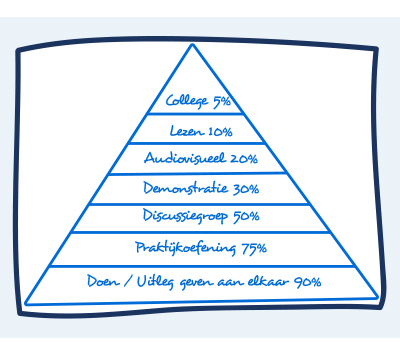
\includegraphics[width=4in]{piramidevanbales}
	\caption{Piramide van Bales.}
\end{figure}

Daarbij wil ik verschillende thema's afgaan: colleges, hoe ``leuk'' een les is, het tempo, persoonlijke begeleiding, plenaire of klassikale momenten en taken opgegeven door een docent. Vooral de colleges en klassikale momenten vond ik interessant om onder de loep te nemen omdat volgens de leercone van Dale die heeft geleid tot de leerpiramide van Bales, colleges tot zeer weinig retentie zou leiden \cite{leerpiramidebales}. De illusie dat er maar 5\% wordt opgevangen bij een college volgens de leerpiramide van Dale is in duigen gevallen door verschillende onderzoeken samengevat door Lalley \& Miller, die aantonen dat het wel degelijk aangetoond tot retentie kan leiden \cite{lalley2007learning}. Zoals alles in context en doel belangrijk.

\subsection{Methodiek}
Aan de hand van een vragenlijst die beschreven staan in \hyperref[sec:vragenlijstRP]{Bijlage E - Vragenlijsten} heb ik geprobeerd te kijken wat de verschillen zijn tussen studenten en docenten door dezelfde onderwerpen vragen in een vraag geformuleerd voor de student en één geformuleerd voor de docent. Het is niet een wetenschappelijk opgestelde vragenlijst, noch zal de analyse een wetenschappelijke aard hebben.

De vragen zijn op een schaal van nooit-altijd beantwoord. Bij sommige van de vragen heb ik alle antwoorden die positief/negatief zijn bij elkaar gegooid het onderscheid daartussen iets scherper te krijgen.

Voor de studie heb ik het woord ``leuk'' gebruikt in de vragenlijst, daar vallen mensen wellicht over, maar het belangrijkste is naar mijn mening dat de interesse gewekt is en er een urgentie-besef is voor de student die intrinsieke motivatie oplevert om zelf te leren zoals Dochy beschrijft in de HIL(L)-methode \cite{dochy2015high}.

\subsection{Bevindingen}
Ten eerste is mij duidelijk dat de vragen die ik heb gesteld niet altijd duidelijk waren, en in sommige opzichten onvolledig. Dus ik zal het even moeten doen met de vragen die gesteld zijn. 

\subsubsection{Colleges}
Eigenlijk zijn zowel studenten (92.6\%) en docenten (100\%) het er mee eens dat de colleges meer dan soms nuttig zijn. Opvallend is dan wel dat bijna de helft van de studenten (43.1\%) vindt dat zij overwegend niet veel hoeven in te halen als ze een college gemist hebben, terwijl de docenten (90\%) dat overwegend wel vinden.

\subsubsection{``Leuk'' (ofwel intrinsieke motivatie)}
Alle docenten proberen over het algemeen het vak leuk te maken (100\%), de meeste studenten (87\%) vinden dat een docent daar ook in bepalend kan zijn voor een vak. En daarin hebben juist docenten (100\%) vaker het idee dat dat effect heeft dan studenten (92\%).

\subsubsection{Tempo}
Het meest verdeeld lijken de studenten en docenten over het tempo van de les. Als een docent te snel gaat dan haakt 51.3\% soms niet/wel, 18.8\% vaak en 8.8\% altijd af. Terwijl als een docent te langzaam gaat haakt 50\% soms niet/wel, 18.8\% vaak en 11.3\% altijd af.

Het lastige hierbij is dat van de docenten 61\% aangeeft niet altijd door te hebben dat ze te snel gaan en daarmee de studenten af haken. En ongeveer evenveel (60\%) docenten aangeven niet altijd gas terug te nemen als ze te snel gaan.

\subsubsection{Persoonlijke begeleiding}
De meeste studenten (93.6\%) zoeken zelf iets uit als iets niet snappen, waarbij ook de meesten meestal om hulp vragen als ze er niet uitkomen (93.9\%), dit komt ook wel overeen met hoe de docenten er naar kijken. Het overgrote gedeelte laat de studenten zelf ploeteren (88.9\%) terwijl de meeste ook denken dat een student om hulp vraagt als een student er niet uitkomt (93.4\%).

Van de studenten geeft 10.1\% aan dat het meestal niet helpt als een docent bij ze komt zitten om iets uit te leggen, terwijl geen een van de docenten dit lijkt in te zien (0\%!).

\subsubsection{Klassikaal}
De klassikale momenten van uitleg zijn in onze ``flipped classroom'' inmiddels niet zo heilig meer, maar toch denkt 94.4\% van de docenten dat het meestal duidelijk is na een klassikale uitleg. Terwijl 26.3\% van de studenten vinden dat ze meestal niet veel leren als een docent iets klassikaal uitlegt. Met nog eens 40\% van de studenten die dat ze meestal iets leren, maar niet altijd.
Wat wel opvallend is is dat er ook maar minder dan de helft studenten meeschrijven met een docent, slechts 46.2\% van de studenten geeft aan soms of meestal mee te schrijven.

\subsubsection{Docent geeft opdracht om aan te werken}
Alle docenten vinden dat wanneer ze studenten aan het werk zetten de studenten veel leren, de meeste studenten 89.7\% vinden ook dat dat meestal het geval is.

\subsection{Conclusie \& Discussie}

Onderzoek vertelt ons dat een docent hoeft maar op een manier instructies hoeft te geven en het heeft al een positief leereffect, toch zijn er dingend die meer effect lijken te hebben \cite{hattie2008visible}. Zo zijn momenten van 1-op-1-begeleiding en studenten zelf laten beoordelen en uitleggen een aantal uitspringers volgens onderzoek \cite{schneiderVariables, hattie2008visible}.

Maar wat zijn nou dingen die opvallen in deze resultaten omdat ze zo verschillend worden bekeken door student en docent?

In de resultaten komen een aantal grote verschillen naar voren bij de onderwerpen: colleges, tempo en de klassikale momenten. Misschien ook wel de meest ingewikkelde moment om te faciliteren, sommige mensen lopen voor anderen weer achter.

Een meer merkwaardig resultaat is misschien wel dat iedereen het erover eens is dat de colleges wel zin hebben, maar dat student en docent er heel anders naar kijken hoeveel het werk er in te vallen valt na een gemiste les. Docenten zeggen allemaal dat er hier wel werk bij komt kijken, terwijl 43.1\% van de studenten, dat gevoel niet lijkt te delen. Wellicht houden het tempo en de `nuttigheid' van de colleges ook wel met elkaar verband. In ieder geval wil ik speculeren dat ze verband houden met feit dat een kwart van de studenten aangeven niet iets te leren van een klassikale uitleg. Het zal hier voor de studenten niet helpen dat ze overwegend niet meeschrijven. Dit zal de retentie en het leereffect van de colleges zeker helpen.

De docenten geven aan niet gas terug te nemen, terwijl ze door hebben dat ze te snel geven en de studenten geven aan dat ze dan niet meer betrokken zijn bij de les. Het aantal studenten wat afhaakt als het te langzaam gaat zit ongeveer rond hetzelfde percentage. Hoe kan een docent hier rekening mee houden? Een klassikaal moment is natuurlijk ook lastig, veel niveauverschillen. In die zin kan je nooit iedereen tevreden houden. Maar toch zou men als docent graag hier in iets willen betekenen voor de studenten. Een conclusief en finaal antwoord kan ik hier niet voor bieden. Wel heb ik een manier gevonden waarin ik het idee heb dat ik invloed kan uitoefenen op de participatie in de les.

\subsubsection{Suggesties voor de participatie }
Aan het begin van een lesperiode (na ongeveer 2 á 3 weken in een lesperiode van 2 maanden) probeer ik graag te polsen hoe de lesstof en de lessen worden ervaren aan de hand van een korte vragenlijst, ik vraag hierin ook om tips en wat ze graag anders zouden willen zien. De resultaten van deze korte vragenlijst bespreek ik tijdens de les met de studenten. Ik heb het idee dat ik hiermee een gevoel van inspraak en zeggenschap kan creëeren terwijl ik ook mijzelf open stel voor verbetering. Wanneer hier ruimte voor is krijg ik het idee dat er ook wederzijds ruimte is voor feedback op de les, maar ook op het leren. Dan probeer ik aan te geven wat strategieën zijn die werken, en op wat voor beoordeling ze af stevenen als het zo verder gaat.

Als ik ook kijk naar de beoordelingen van de studenten, de participatiegraad, de aanwezigheid en de eindcijfers, dan denk ik dat ik boven het gemiddelde heb gescoord de afgelopen periode waar ik dit gesprek ben aangegaan. Nou is het altijd lastig aan te geven waardoor dit nou precies komt, maar ik denk zeker als docent ook daarin mijn stempel te hebben kunnen drukken. 


\bibliography{portfolio.bib}
\clearpage
\begin{appendices}

\section{Reflectie Lesdemo}
\label{sec:lesdemo}
Voor de lesdemo heb ik niet een bestaande les gepakt omdat dat niet zou aansluiten bij de voorkennis van de medestudenten in de Didactiekcursus. De les die ik gemaakt had was een korte introductie op een aantal begrippen in het programmeren met opdrachten die zelf uitgevoerd konden worden op ieders laptop. Zelf had ik het idee dat ik veel aan het woord was een kwaal die mij vaker overkomt. En dat ik soms wat te veel gas geef in de les. Ik wil graag dat iedereen erbij is. Daarbij geef ik dan heel veel energie met vragen als: \textit{"Is iedereen er nog bij? Kan ik verder"}, etc. Naar mijn idee komt dat nogal onrustig en opzweperig over. Bovendien houd ik dat ook niet lang vol. Een collega van mij verwoorde het zo:
\begin{quotation}
  \textit{"Ik zie dan Fritz de bandleider, dat mag echt wel rustiger. Het is geen concert."}
\end{quotation}
In de feedback van mijn medestudenten waren de overtonen positief: \textit{heel relaxed, op je gemak, leuk om mee te doen, goed gebruik van je stem, natuurlijk overwicht, goed gebruik van complimenten, enthousiast}. De tips zaten wat meer op de context en protocol: \textit{waar doen we dit voor, de transfer is niet helder, het mist wat structuur (wat, waarom en hoe), context ontbreekt.}
Kort gezegd miste de les wat omlijsting. Dit is een bekende valkuil van mij. Dit heeft ook bijgedragen aan het vormen van het leerdoel voor het onderdeel \textit{Activerende didactiek}. Voor de lessen neem ik mee dat ik wat meer ondertiteling wil geven aan het proces. Als ik bijvoorbeeld de studenten aan de slag laat met elkaars werk nakijken, geef ik daarbij aan dat ik dat bewust doe omdat ze er minder van zouden leren als ik het voordoe, dan wanneer ze er met elkaar over bakkeleien.
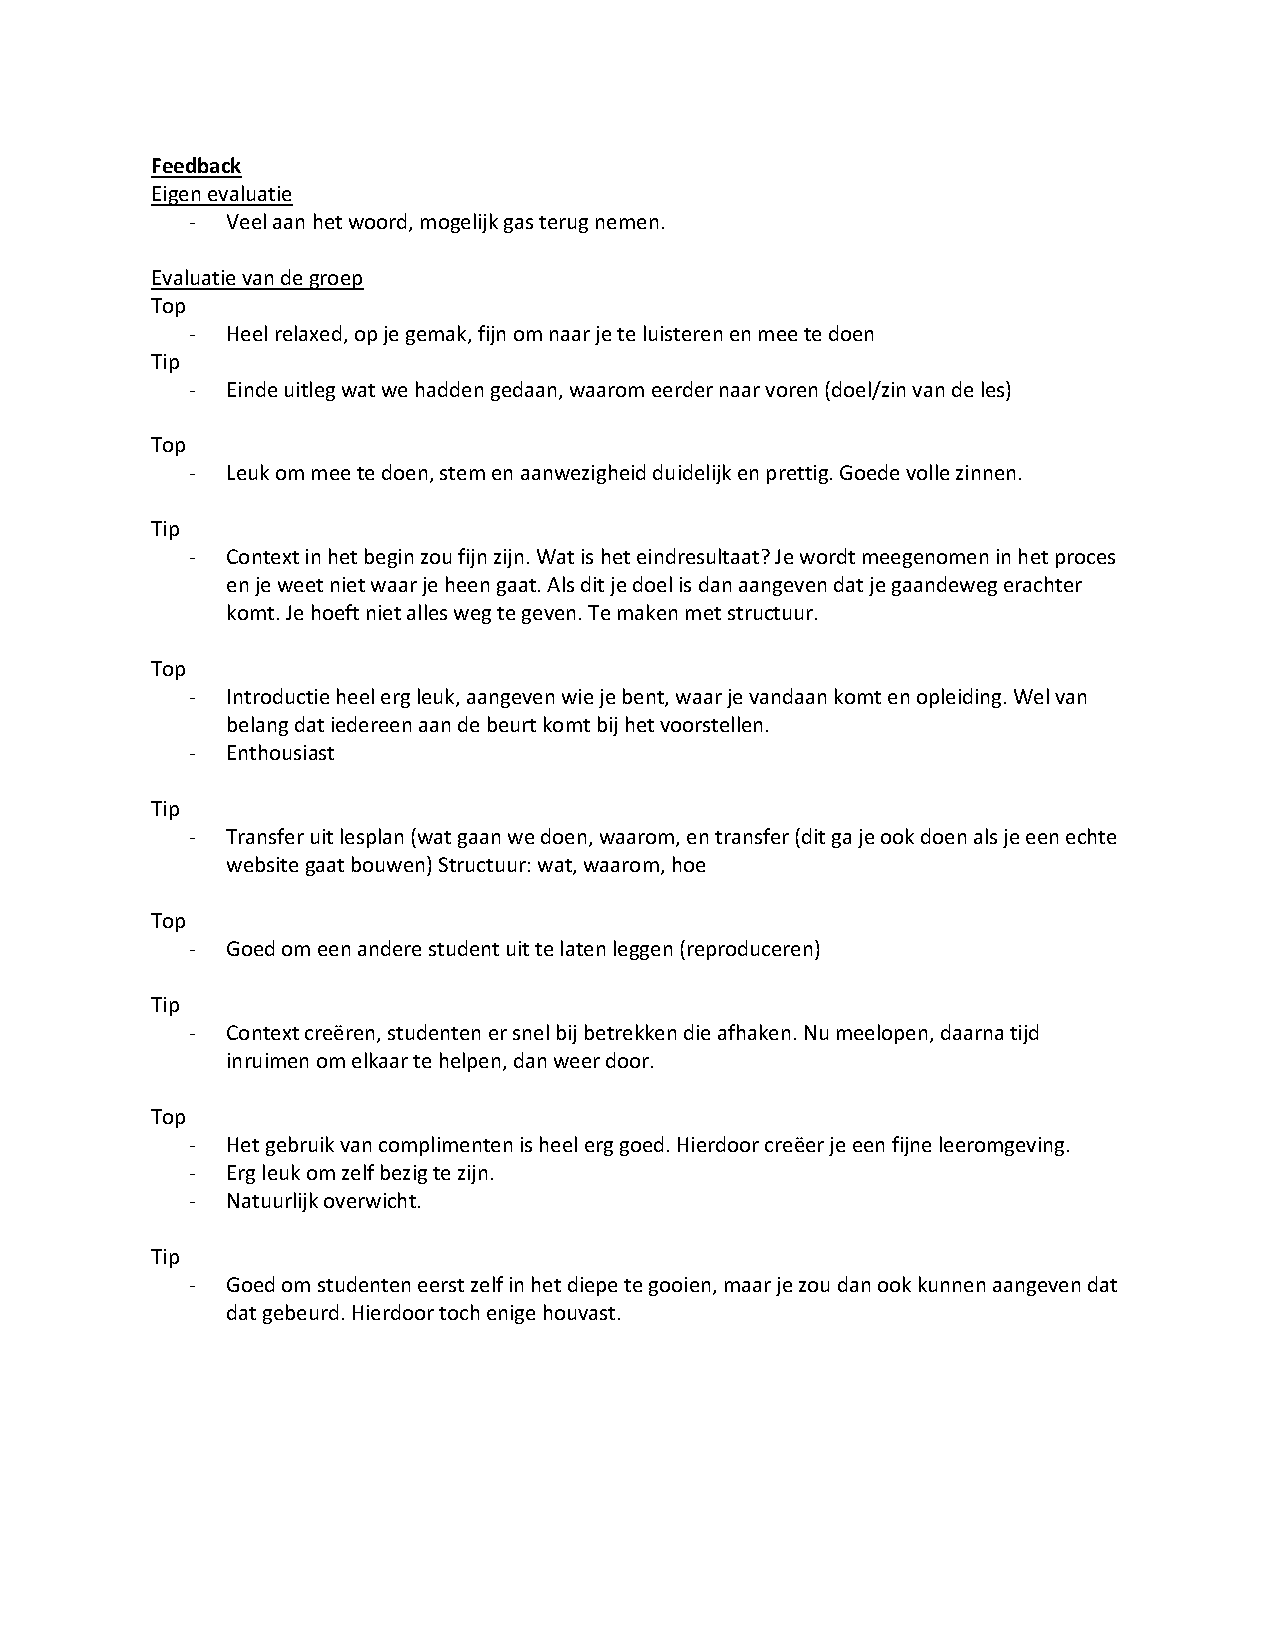
\includepdf[pages=-]{FeedbacklesdemoFritz22-5.pdf}


\section{Reflectie Lesbezoek Docent VDO}
\label{sec:lesbezoek}
De les die bezocht werd viel precies binnen de periode dat ik ook bezig was met mijn leerdoel: 4x een les voorbereiden aan de hand van een lesplan. Die lessen gingen ook heel erg goed. Zelf kreeg ik het idee dat ik soms weinig \textit{witruimte} laat tijdens de les. Elk moment is ingevuld. Soms kan ik de studenten best even ruimte geven om even na te denken en zelf te besluiten wat ze gaan doen. Tijdens de les deed ik achter elkaar:
\begin{itemize}
  \item een intro op de les
  \item kahoot
  \item duo's overleggen
  \item codedemo

\end{itemize}
Achteraf gezien had ik deze beter kunnen uitsmeren over de les.

Ongeacht mijn eigen gevoel over de les, kreeg ik overwegend positieve feedback van Lia. Met de kanttekening dat ik de didactiek en het proces meer mag benoemen tijdens de les. Of een vraag zou kunnen doorspelen naar een andere student in plaats van als docent de alwetende Ivoren Toren spelen. 
Verder is de feedback positief. De dingen waar ik op kan letten neem ik mee.

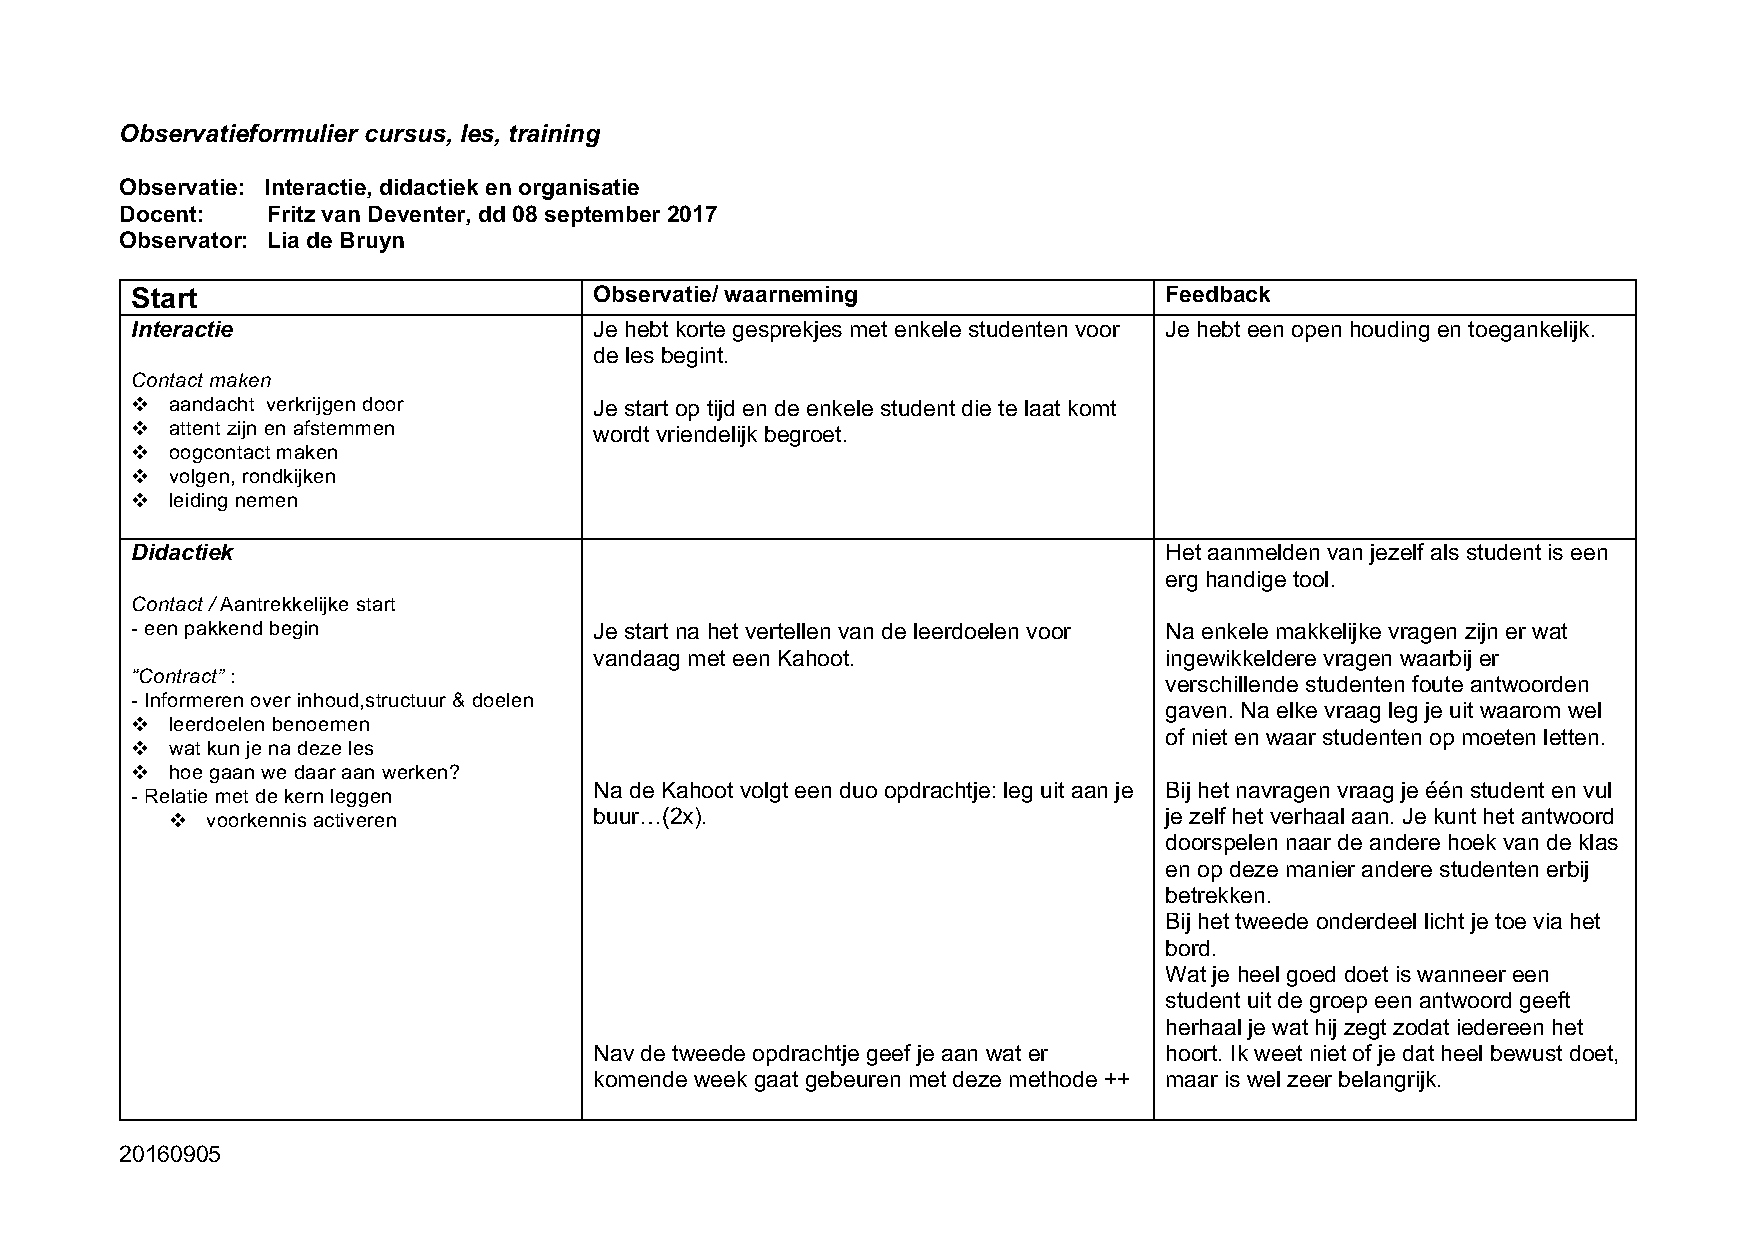
\includepdf[pages=-]{ObservatieLia.pdf}

\section{Reflectie Lesbezoek Collega: Carmen}
\label{sec:lesbezoekcollega}
De les waar Carmen bij zat, was een klein beetje een vreemde, omdat deze altijd na een hele drukke les de dag daarvoor valt. Over het algemeen laat ik de studenten tijdens deze les iets meer zelfstandig werken, zodat ze een beetje kunnen bijwerken wat ze misschien nog niet hebben kunnen doen tijdens de rest van de week.

Desalniettemin ging de les aardig zoals ook te zien is in het commentaar van Carmen. Zij noemt eveneens als Lia ook dat de opstelling (bus-opstelling) misschien ook iets afdoet aan de interactie die er anders zou kunnen zijn.

Daarnaast wordt wederom aangekaart dat er in mijn lessen soms dingen onduidelijk zijn omdat ik ze niet verschaf van een inleiding. Soms vergeet ik ook het doel of de tijd die ze ergens voor hebben uit te leggen, dat komt hier ook weer naar voren in de observatie van Carmen.

Als ik iets uitleg zou ik ook een student kunnen vragen om op het bord te tekenen/schrijven, dat doe ik nu vaak zelf.

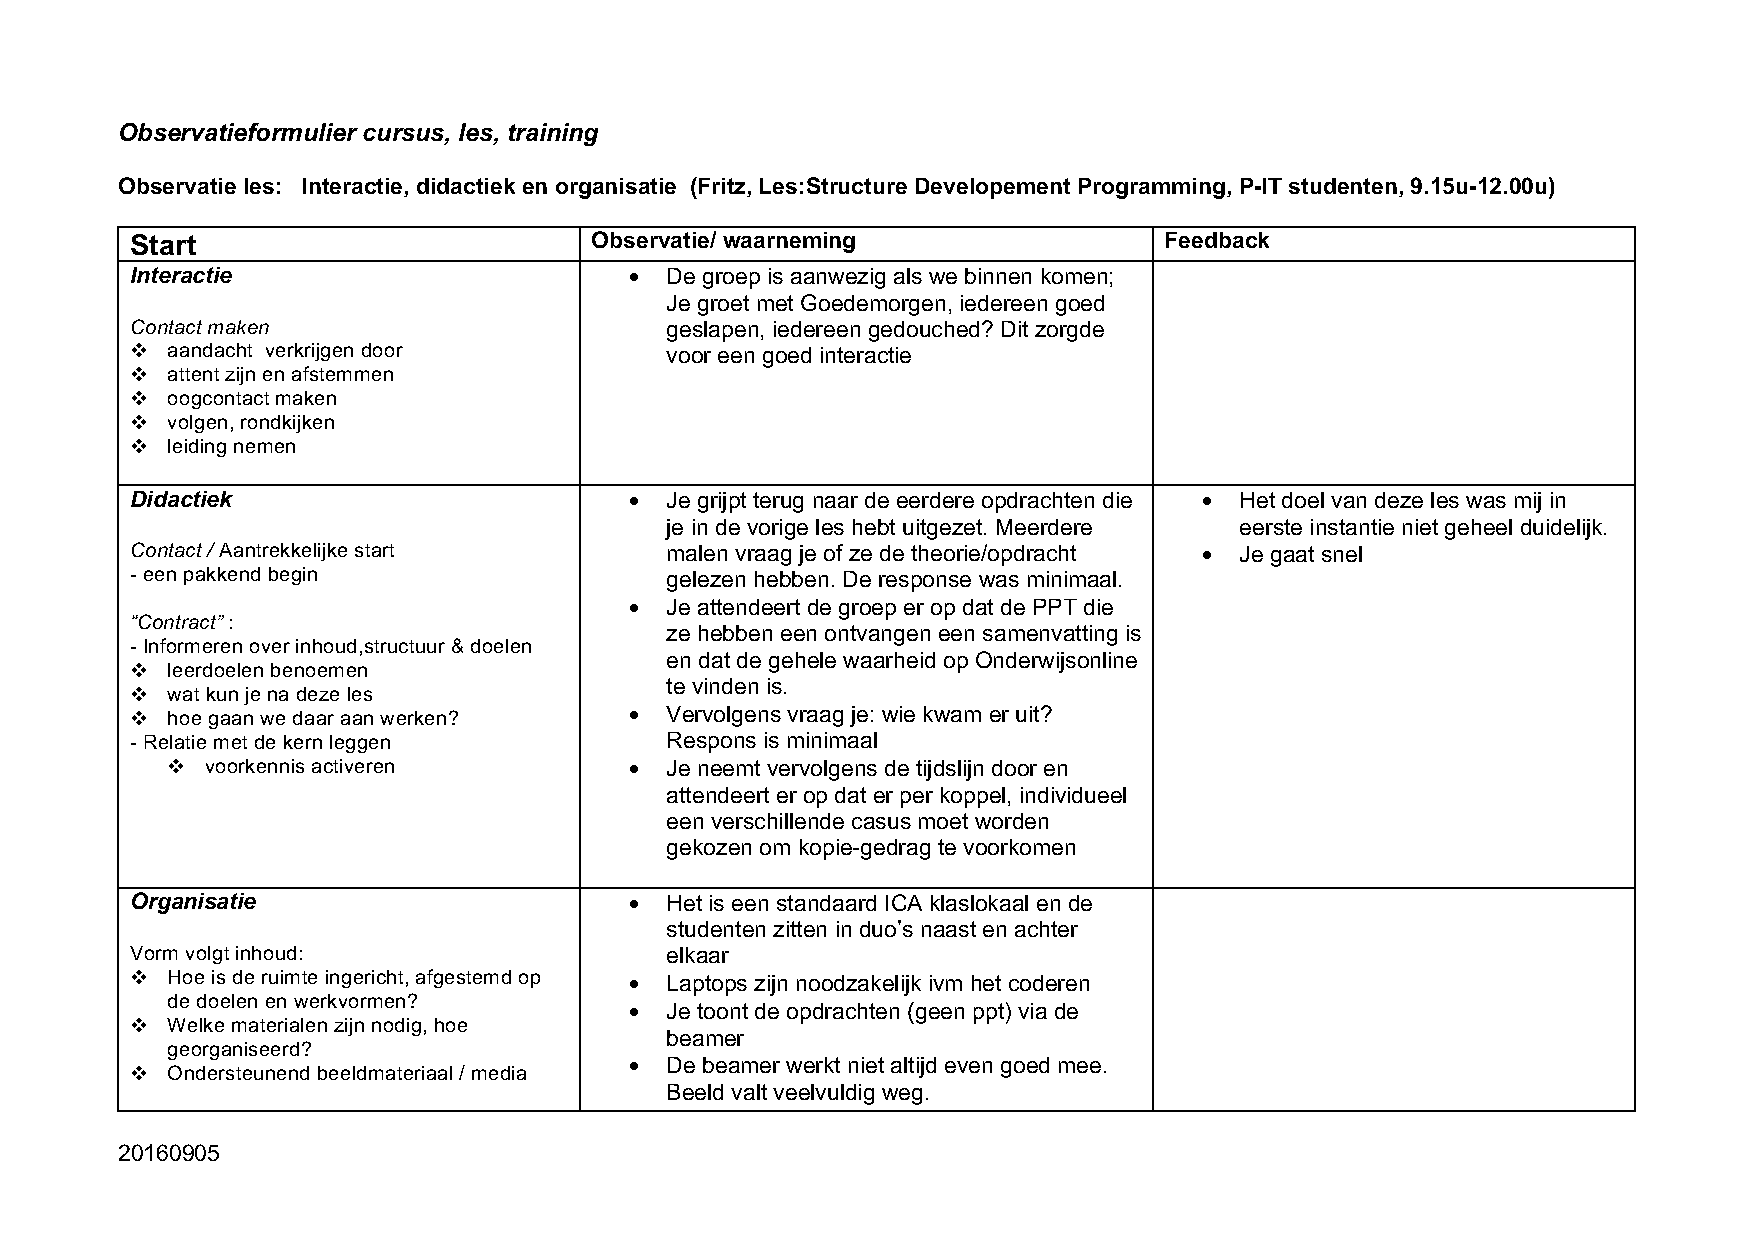
\includepdf[pages=-]{ObservatieCarmen.pdf}


\section{Situatieschets Groepsbegeleiding}
\label{sec:groep}
\subsection{Context}
In het eerstejaars project van de Informatica opleiding (I-Project) ben ik procesbegeleider geweest van een groep studenten die een veilingssite moesten maken voor een opdrachtgever (een rol die vervuld werd door een andere docent). De casus en de inhoud van de opdracht waren weggelegd voor de opdrachtgever. Het was belangrijk dat het groepje waar ik begeleiding aan gaf bekend zou worden met de procestool: \textit{Scrum}. Scrum is een manier van werken in teamverband waar er getracht wordt kleine iteraties te maken die elk afgerond worden met een product wat af is. In de praktijk betekent dit veelal het afspreken, plannen en opleveren van de beloofde dingen voor een product in een tijdsperiode van een aantal weken, een zogenoemde \textit{sprint}. Na afloop van elke sprint is er normaliter een \textit{retrospective}, een overleg met elkaar om terug te blikken op hoe het samenwerken gegaan is. Naast dit overleg kwam ik regelmatig langs om even te kijken hoe het ging (en of iedereen wel aanwezig is).

\subsection{Situatie}
In de groepsgesprekken gaf ik meestal een taak mee voor het volgende ontmoetingsmoment. De opdracht die ik gegeven had voor dit specifieke gesprek was om feedback op te schrijven voor elk van de groepsleden, een tip en een top. De opdracht had ik gegeven omdat in sommige van de gesprekken daarvoor ze ook de taak hadden om feedback mee te nemen, maar de meesten deden het uit het hoofd en het leek nogal verzonnen ``on-the-spot``, het had weinig diepgang en iedereen ging elkaar wat napraten. Ik had nadrukkelijk genoemd dat iedereen echt wat moest opschrijven, anders zou ik zelf weglopen bij het gesprek, omdat het dan ook geen zin had om feedback met elkaar te bespreken.

De volgende afspraak had iedereen wat opgeschreven en meegenomen. Toen we de ronde deden was een van de leden van de groep (we geven hem even de fictieve naam: Hendrikus) nog steeds terughoudend met het geven van de tip. Hendrikus noemde steeds dat de anderen het zo goed doen en dat hij er niet echt iets had op aan te merken. Op dat moment leek het mij verstandig om een zijstapje te doen en te communiceren over het communiceren met de groep. Ik vroeg ze of ze het prima vonden als Hendrikus iets over hun zou zeggen waar ze aan moesten werken of wat niet louter positief was. De groep antwoordde dat ze daar echt niet bang voor waren, dit verwoordde ze ook naar Hendrikus, dat hij zich daar niet zorgen over hoefde te maken. Ik vroeg ook Hendrikus of hij misschien wist waarom hij het niet zo goed over zijn lippen kreeg. Had hij dan geen feedback? Of vond hij het spannend? 

Op dat moment leek het alsof er even een schilletje om Hendrikus wegviel. Hij noemde dat hij het inderdaad ingewikkeld vond om iets negatiefs (ook al was het opbouwend bedoeld) te zeggen omdat hij in zijn schoolloopbaan redelijk veel gepest werd. Hij was bang dat hij het vertrouwen of zijn goede band met de anderen zou schaden door iets te noemen wat niet positief was. Nadat hij dit noemde reageerde de groep accepterend en herhaalde nogmaals dat hij zich er niet zorgen om hoefde te maken. Waarna Hendrikus ook zijn tips durfde te delen.

Wat ik merkte in dit gesprek is dat het echt wel loont om soms even een zijstap te doen en te durven door te vragen. Wat er nog wel bij gezegd moet worden, is dat in deze groep een andere jongen de groep heeft moeten verlaten die kampte met depressie in combinatie met een Autisme Spectrum stoornis.

\section{Situatieschets Individuele begeleiding}
\label{sec:individu}
Één van de studenten die ik begeleid voor zijn afstuderen had een projectplan opgestuurd wat nogal onder de maat was. Erg algemene risico's niet echt specifieke doelen om te behalen en onderzoeksvraag waar niet echt mee gewerkt kon worden. Naar aanleiding van zijn projectplan en om even kennis te maken met de student, het afstudeerbedrijf en zijn begeleiders had ik een afspraak gemaakt met hem.

De afspraak begon helaas een beetje scheef omdat ik vergeten was de feedback die ik voor hem had verzameld een aantal dagen voor de afspraak naar hem te sturen. De student was een beetje verrast door mijn terugkoppeling op zijn document en de onderdelen die ik nog te onduidelijk vond. Het overviel hem even op dat moment, dat was totaal niet mijn bedoeling. 

Daarna heb ik geprobeerd door wat vragen te stellen duidelijker te krijgen wat de situatie was en wat de doelstelling van de opdracht was. Op een gegeven moment heb ik het gesprek afgerond en voorgesteld om nog even met de student individueel te zitten en samen te kijken naar de onderzoeksvraag en het werk wat er nog moet gebeuren.

De gesprekstechnieken die besproken zijn in de lessen en de oefening met de acteur waren mij allemaal even ontschoten en het kostte mij redelijk wat tijd om die weer op orde te krijgen. De taak als begeleider is naar mijn idee om de student zelf aan het denken te zetten. Op het moment dat de situatie dan geheel anders loopt, doordat de student de feedback pas voor het eerst hoorde toen ik bij hem was, dan is het toch een stuk lastiger om het ook daadwerkelijk bij de student te laten en niet zelf heel hard te gaan werken. 

Gezamenlijk hadden we afgesproken om elkaar nog telefonisch te spreken over het projectplan een week later. Tijdens dat gesprek was het een stuk makkelijker om de "goede" vragen te stellen en de student aan het werk te zetten. Hier blijkt voor mij duidelijk uit dat het belangrijk is om die gesprekstechnieken veelvuldiger te oefenen en te gebruiken zodat het een tweede natuur wordt, ook voor de onvoorziene situaties.


\section{Vragenlijsten}
\label{sec:vragenlijstRP}
\subsection{Voor studenten}
\begin{itemize}
  \item Wat is uw geslacht?
  \item In welke leeftijdscategorie valt u?
  \item Ik kom naar de colleges
  \item Ik vind de colleges nuttig
  \item Als ik een college mis, moet ik veel stof inhalen
  \item Een docent is heel bepalend in hoe leuk het vak wordt
  \item Als een docent leuk is leer ik meer
  \item Als een docent te snel gaat haak ik af
  \item Als een docent te langzaam gaat haak ik af
  \item Als ik iets niet snap, stel ik een vraag
  \item Als ik iets niet snap, zoek ik zelf uit hoe iets werkt
  \item Als ik er dan nog niet uitkom vraag ik om hulp
  \item Als een docent even bij mij komt zitten dan helpt dat
  \item Als een docent klassikaal iets uitlegt leer ik veel
  \item Als een docent klassikaal wat uitlegt schrijf ik mee
  \item Als een docent mij aan het werk zet leer ik veel
  \item Als ik een oefentoets (zelf) maak leer ik veel
  \item Ik leer het beste als ik alle stof in 1 keer hoor en het 1 keer doe
  \item Ik leer het beste als de stof wat wordt uitgespreid en ik elke dag even oefen
\end{itemize}

\subsection{Voor docenten}
\begin{itemize}
  \item Wat is uw geslacht?
  \item In welke leeftijdscategorie valt u?
  \item Aanwezigheid van de colleges is raadzaam
  \item Het college is nuttig
  \item Als een student een college mist, moet deze veel inhalen
  \item Ik probeer het vak leuk te maken
  \item Een leuke les of docent maakt veel uit voor het leereffect
  \item Soms ga ik te snel en haken studenten af, daar ben ik mij bewust van
  \item Soms ga ik te snel en haken studenten af, ik probeer dan gas terug te nemen
  \item Er worden vragen gesteld in mijn lessen
  \item Ik laat de studenten graag zelf even ploeteren
  \item Er wordt mij om hulp gevraagd als een student er niet uitkomt.
  \item Het heeft effect als ik bij een student kom zitten voor hulp
  \item Als ik klassikaal iets uitleg is het duidelijk
  \item Studenten staat het vrij om mee te schrijven
  \item Als ik de studenten aan het werk zet leren ze meer
  \item Als studenten een oefentoets maken leren ze veel
  \item Ik geef het liefste in 1 keer een hele bak theorie
  \item Ik geef het liefst een bak theorie uitgespreid over de week heen
\end{itemize}


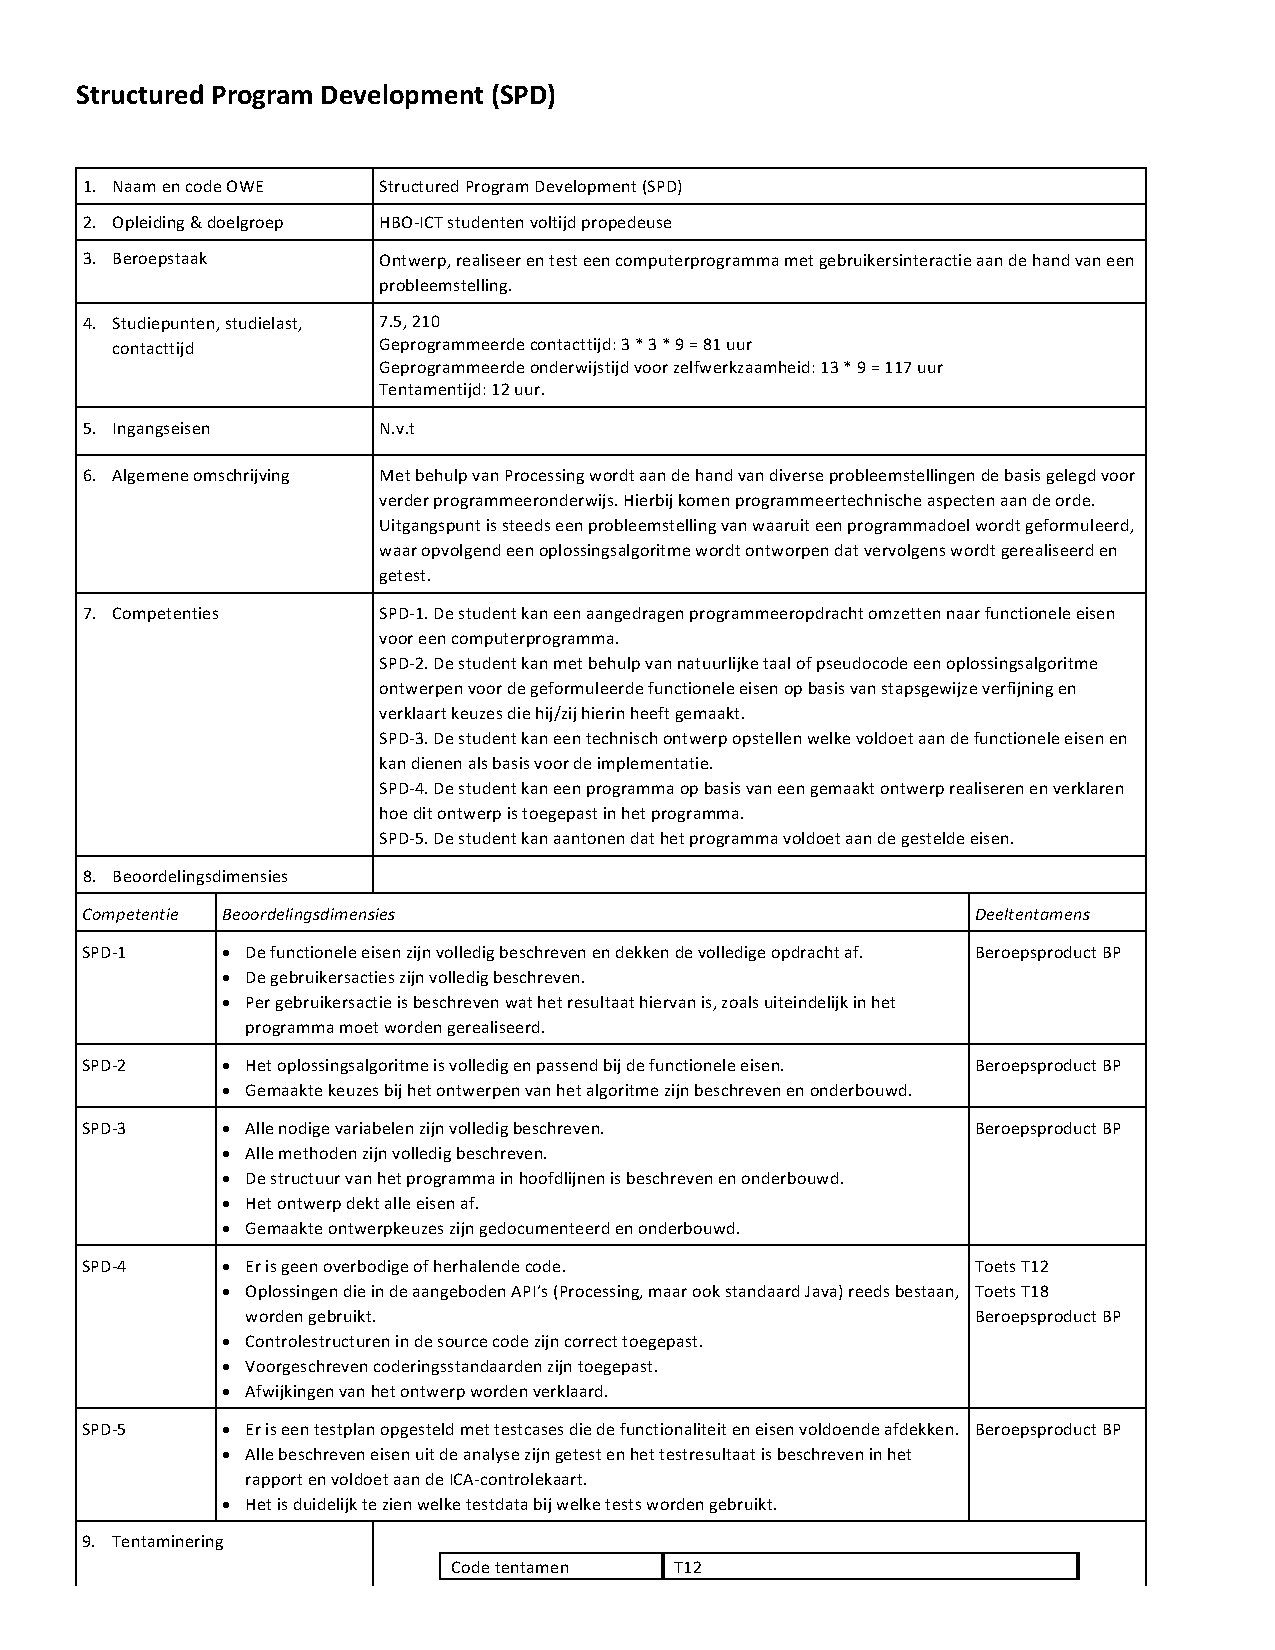
\includepdf[pages=-,pagecommand={\addcontentsline{toc}{section}{\protect\numberline{F}OWE voor vak SPD}\label{sec:owespd}}, fitpaper=true]{OWE-SPD.pdf}

\end{appendices}

\end{document}
